\textbf{\subsection{Расчет предоконечного каскада}}
\vspace{1em}

Предоконечный каскад, как и входной, являются усилителями напряжения до уровня, необходимого в непосредственном усилителе мощности, выполненном на оконечном каскаде, а также для согласования входного сигнала с входом оконечного каскада. Поэтому в предоконечном каскаде не ставится задача усиления мощности и он работает в режиме А, с КПД порядка 25\%. В этом режиме ток в выходной цепи протекает в период всего действия сигнала. Режим А дает возможность получения максимальной амплитуды выходного сигнала с минимальными искажениями. Воздействие на низкоомную нагрузку RН сигнала большой амплитуды приводит к значительному увеличению КПД усилителя и его мощности.
За счет включения в коллекторную цепь предоконечного каскада, выполненного по схеме с общим эмиттером, динамической нагрузки получаем большой коэффициент усиления по напряжению. \par
Каскад охвачен местной положительной ОС, что дает возможность увеличения коэффициента усиления K, но уменьшения полосы пропускания.\par

\begin{figure}[!htbp]
    \center{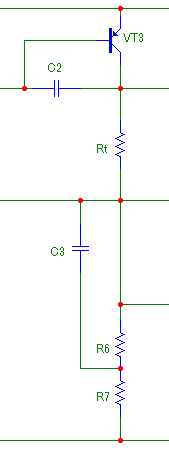
\includegraphics[width=0.23\linewidth]{picture_pk}}
    \caption{Схема предоконечного каскада}
    \label{figure:p2_4}
  \end{figure}

Таким образом, основные особенности каскада предварительного усиления в том, что за счет работы в режиме А, он обеспечивает минимальные искажения, при достаточно усилении амплитуды сигнала. Включение в выходную цепь динамического сопротивления позволяет увеличить коэффициент усиления K в десятки раз.\par


\subsubsection{Ток покоя транзистора VT3:}

\begin{equation}
\label{eq:equation3_1}
 I_{\text{O К3}} = (2\ldots 3)\cdot I_{\text{Б m4}}  = (2\ldots 3)\cdot I_{\text{нм}}/h_{\text{21 экв}}
\end{equation}
\begin{equation*}
  I_{\text{O К3}} = \dfrac{2.5 \cdot 2.83 }{ 400 } = 0.02
\end{equation*}
 
 \subsubsection{Выбор резистора R7:} 
 
\begin{equation}
\label{eq:equation3_2}
R_{7} = (30\ldots 50)\cdot R_{н} = 40 \cdot 2 = 80~\text{Ом}
\end{equation}
Резистор R7 включается в цепь для того, чтобы не закорачивать источник питания конденсатором С3, обеспечивающим включение в выходную цепь транзистора динамической нагрузки R6. Основное усиление напряжения происходит за счет динамической нагрузки R6, потому резистор R7 выбирается малой величины.

\subsubsection{Выбор резистора R6:} 
\begin{equation}
\label{eq:equation3_3}
 R_{6} = (E_{0} - U_{\text{БЭ5}} - I_{\text{О К3}} \cdot R_7)/I_{\text{0 К3}} = (17 - 0.6 - 0.023 \cdot 80)/0.02 = 728~\text{Ом}
\end{equation}

При прохождении сигнала динамическое сопротивление R6 будет определяться:
\begin{equation}
\label{eq:equation3_4}
  R_{\text{6Д}} = \dfrac{R_6}{1-K_{\text{ОК}}} = 10 \cdot 728 = 7280~\text{Ом}
\end{equation}

Коэффициент усиления оконечного каскада $K_{\text{ОК}}$, т.к. он является повторителем напряжения, близок к 1 и составляет более 0.9: $K_{\text{ОК}}$ = 0.9. \par
С обеих сторон резистора R6 потенциалы близки за счет того, что цепь термостабилизации не вносит особо падения напряжения и транзисторы VT4 и VT5 являются повторителями напряжения. Ввиду этого на обоих концах установятся близкие потенциалы, т.е. разность потенциалов будет очень мала и ток практически не будет протекать. Что эквивалентно включению большого сопротивления. За счет этого происходит увеличения коэффициента усиления. \par

\subsubsection{Определение емкости C3:} 
Эта емкость устраняет протекание переменного тока по цепи R6 – R7 – земля и увеличивает коэффициент усиления каскада. Обеспечивает связь транзистора VT3 с нагрузкой R6 через оконечный каскад. \par
\begin{equation}
\label{eq:equation3_5}
  C_3 \geq \dfrac{5 \ldots 10}{2 \pi f_{\text{н}} (R_7 + R_{\text{н}})} \geq \dfrac{5}{2 \pi 10 (80 + 2)} \geq 970~\text{мкФ}
\end{equation}

\subsubsection{Параметры выбора транзистора VT3:}
\begin{equation}
\label{eq:equation3_6}
P_{\text{к доп}} = (1.2 \ldots 1.5) P_{\text{к 3}} = (1.2 \ldots 1.5) \cdot \dfrac{E_0 I_{\text{0 кз}}}{2} = 1.3 \cdot \dfrac{17 0.02}{2} = 0.221~\text{Вт}
\end{equation}

\begin{equation}
\label{eq:equation3_7}
I_{\text{к 3m}} = I_{\text{О КЗ}} + \dfrac{I_{\text{нм}}}{h_21} = 0.013 + \dfrac{2.83}{400} = 0.020~\text{А}
\end{equation}

\begin{equation}
\label{eq:equation3_8}
I_{\text{к доп}} = (1.2 \ldots 1.5) I_{\text{к 3m}} = 1.3 \cdot 0.020 = 0.026~\text{А}
\end{equation}

\begin{equation}
\label{eq:equation3_9}
U_{\text{кэ доп}} = (1.2 \ldots 1.5) E_{\text{0}} = 1.3 \cdot 17  = 22.100~\text{В}
\end{equation}

\begin{equation}
\label{eq:equation3_10}
f_{h_{21}} = (2 \ldots 3) f_{\text{в}} = 2.5 \cdot 18000 = 45~\text{кГц}
\end{equation}

Параметр h21 выбирается из максимально возможных по заданным параметрам.

\begin{table}[htbp]
\caption{Характеристики выбранного транзистора в ПОК}
\begin{center}\begin{tabular}{|c|c|c|c|c|c|c|}
\hline 
  & тип & $P_{\text{к}}$ доп, Вт & $I_{\text{к}}$ доп, А & $U_{\text{к}}$ доп, В & $h_{21}$ &  $f_{h_{21}}$, кГц \\ 
\hline 
VT4 & n-p-n & 3.66  & 3.11 & 19 & 400 & 36.00\\ 
\hline 
\end{tabular} 
\end{center}
\end{table}

\subsubsection{Расчет цепи смещения:}

Схема цепи смещения на транзисторах представлена на рисунке 2.4. \par
Находим ток делителя:
\begin{equation}
\label{eq:equation3_11}
 I_{\text{д}} = (0.1 \ldots 0.3) I_{\text{0кз}} = 0.2 \cdot 0.02 = 0.04~\text{А}
\end{equation}

Выбор VTt практически определяется допустимым током
\begin{equation}
\label{eq:equation3_12}
 I_{\text{к доп}} = (1.1 \ldots 1.3) I_{\text{к3max}} = 1.2 \cdot 0.024 = 0.029~\text{А}
\end{equation}

Определяем $R_{\text{бт}}$ ($U_{\text{бт}} \approx 0,5 - 0,6$ В)
\begin{equation}
\label{eq:equation3_13}
 R_{\text{бт}} = U_{\text{бт}} / I_{\text{д}} = 0.5/0.029 = 17~\text{Ом}
\end{equation}

Сопротивление подстроечного резистора
\begin{equation}
\label{eq:equation3_14}
 R_{\text{П}} = 2 (U_{\text{СМ}} - n U_{\text{Д}}) / I_{\text{0 КЗ}} = 2 (1.2 - 0.5) / 0.04 = 35~\text{Ом}
\end{equation}

\subsubsection{Входное сопротивление предоконечного каскада:}
Рассчитаем $R_{\text{ВХ3}}$ и $r_{\text{Э3}}$
\begin{equation}
\label{eq:equation3_15}
 R_{\text{ВХ3}} = h_{\text{11 VT3}} = (1 + h_{\text{21 VT3}}) \psi_T / I_{\text{0 Э3}} = (1 + 80) \cdot 25 / 40 = 51~\text{Ом}
\end{equation}
\begin{equation}
\label{eq:equation3_16}
 r_{\text{Э3}} = \psi_T / I_{\text{0 Э3}} = 25/40 = 0.625~\text{Ом}
\end{equation}

Что соответствует значению входного сопротивления в схеме с общим эмиттером, которое имеет небольшое значение и определяется сопротивлением прямо смещенного эмиттерного перехода, имеющем незначительную величину, в пересчете на малый входной ток базы.

\subsubsection{Коэффициент усиления каскада по напряжению:}

Предоконечный каскад имеет большое усиление по напряжению за счет того, что в коллекторной цепи включена динамическая нагрузка.
\begin{equation}
\label{eq:equation3_17}
 K = \dfrac{R_{\text{КН3}}}{r_{\text{э3}}} = \dfrac{R_{\text{ВХ4}} ( R_{\text{6Д}} + К_7)}{ r_{\text{э3}}} = \dfrac{h_{21} R_{н}}{r_{\text{э3}}}
\end{equation}
\begin{equation*}
  K = (400 \cdot 2) / 0.625 = 1280
\end{equation*}

Входное сопротивление оконечных каскадов состоит из малого входного сопротивления транзистора по схеме с общим эмиттером и сопротивлением, учитывающим влияние местной ООС, тем самым увеличивая входное сопротивление.  Влияние R9 и R10 , ввиду их малости, можно не учитывать. \par

\subsubsection{Итоговые данные предоконечного каскада:}

\begin{table}[htbp]
\caption{Параметры выбора транзистора}
\begin{center}\begin{tabular}{|c|c|c|c|c|c|c|}
\hline 
  & тип & $P_{\text{к}}$ доп, Вт & $I_{\text{к}}$ доп, А & $U_{\text{к}}$ доп, В & $h_{21}$ &  $f_{h_{21}}$, кГц \\ 
\hline 
VT4 & n-p-n & 3.66  & 3.11 & 19 & 400 & 36.00\\ 
\hline 
\end{tabular} 
\end{center}
\end{table}

\begin{table}[htbp]
\caption{Режимы работы транзистора}
\begin{center}\begin{tabular}{|c|c|c|c|c|c|c|c|c|c|c|c|c|}
\hline 
   & $I_\text{0К}$ & $I_\text{0б}$& $U_\text{0Б}$ & $U_\text{0К}$&  $I_{\text{Км}}$  & $I_{\text{Бм}}$& $U_{\text{км}}$, B & $P_{\text{к}}$ & K\\ 
  & мА & мА& В & В & мА & мА & B & мВт & \\
\hline 
КТ127А-1 & 1 & 0.03 & 0.7 & 5 & 50 & 1.66 & 25 & 15 & 0.99 \\
\hline
\end{tabular} 
\end{center}
\end{table}